In this paper, we will benchmark on the following datasets: Bruce \cite{bruce2005saliency}, Judd \cite{judd2009learning}, Cerf \cite{cerf2008predicting}, FT \cite{achanta2009frequency}, and IS \cite{li2013visual}.  Among these 5 datasets, Judd and Cerf only provides fixation ground-truth.  FT only provides salient object ground-truth.  IS provides both fixations\footnote{IS provides raw gaze data at every time point.  We use the following thresholds to determine a stable fixation: min fixation duration: $160 ms$, min saccade speed: $50px/100ms$.} as well as salient object masks.  While Bruce dataset was originally designed for fixation prediction, it was recently augmented by \cite{borji2013stands} with $70$ subjects under the instruction to \emph{label the single most salient object in the image}.
In our comparison experiment, we include the following fixation prediction algorithms: ITTI \cite{itti1998model}, AIM \cite{bruce2005saliency}, GBVS \cite{achanta2009frequency}, DVA \cite{hou2008dynamic}, SUN \cite{zhang2008sun}, SIG \cite{hou2012image}, AWS \cite{garcia2012relationship}; and following salient object segmentation algorithms: FT \cite{achanta2009frequency}, GC \cite{cheng2011global}, SF \cite{perazzi2012saliency}, and PCAS \cite{margolin2013makes}. These algorithms are top-performing ones in major benchmarks~\cite{borji2012salient}.

\begin{figure}[t]
\centering
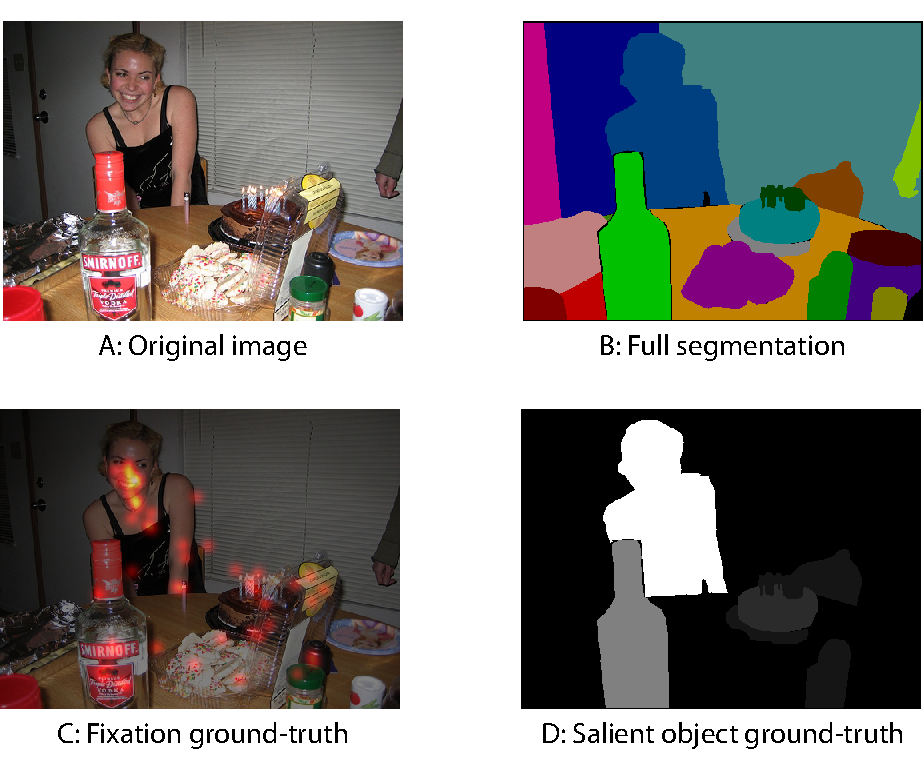
\includegraphics[width=0.7\linewidth]{objLabelGT.pdf}\\
\caption{An illustration of PASCAL-S dataset.  Our dataset provides both eye fixation (Fig.~C) and salient object (Fig.~D) mask.  The labeling of salient objects is based on the full segmentation (Fig.~B).  A notable difference between PASCAL-S and its predecessors is that each image in PASCAL-S is labeled by multiple labelers without restrictions on the number of salient objects.}\label{fig:objLabelGT}
\end{figure}

\subsection{Psychophysical experiments on the PASCAL-S dataset}
Our PASCAL-S dataset is built on the validation set of the PASCAL VOC 2010 \cite{pascal-voc-2010} segmentation challenge.  This subset contains $850$ natural images.  In the fixation experiment, $8$ subjects were instructed to perform the ``free-viewing'' task to explore the images.  Each image was presented for $2$ seconds, and eye-tracking re-calibration was performed on every 25 images.  The eye gaze data was sampled using Eyelink 1000 eye-tracker, at $125Hz$.  In the salient object segmentation experiment, we first manually perform a full segmentation to crop out all objects in the image.  An example segmentation is shown in Fig.~\ref{fig:objLabelGT}.B.  When we build the ground-truth of full segmentation, we adhere to the following rules: 1) we do not intentionally label parts of the image (e.g. faces of a person); 2) disconnected regions of the same object are labeled separately; 3) we use solid regions to approximate hollow objects, such as bike wheels.

We then conduct the experiment of $12$ subjects to label the salient objects.  Given an image, a subject is asked to select the salient objects by clicking on them.  There is no time limitation or constraints on the number of objects one can choose.  Similar to our fixation experiment, the instruction of labeling salient objects is intentionally kept vague.  The final saliency value of each segment is the total number of click it receives, divided by the number of subjects.





\subsection{Evaluating dataset consistency}\label{sec:consistency}
Quite surprisingly, many of today's widely used salient object segmentation datasets do not have any guarantee on the inter-subject consistency.  To compare the level of agreement among different labelers in our PASCAL-S dataset and other existing dataset, we randomly select $50\%$ of the subjects as the test subset.  Then we benchmark the saliency maps of this test subset by taking the rest subjects as the new ground-truth subset. For fixation task, the test saliency map for each image is obtained by first plotting all the fixation points from the test subset, and then filter the saliency map by a 2D Gaussian kernel with $\sigma = 0.05$ of the image width. For salient object segmentation task, the test/ground-truth saliency maps are binary maps obtained by first averaging the individual segmentations from the test/ground-truth subset, and then threshold with $Th=0.5$\footnote{At least half of the subjects within the subset agree on the mask.} to generate the binary masks for each subset.  Then we compute either AUC score or F-measure of the test subset and use this number to indicate the inter-subject consistency.

We notice that the segmentation maps of Bruce dataset are significantly sparser than maps in PASCAL-S or IS. Over $30\%$ of the segmentation maps in Bruce dataset are completely empty.  This is likely a result of the labeling process.  In Borji \emph{et al.}'s experiment \cite{borji2013stands}, the labelers are forced to choose only one object for each image.  Images with two or more equally salient objects are very likely to become empty after thresholding.  Although Bruce is one of the very few datasets that offer both fixations and salient object masks, it is not suitable for our analysis.

For dataset PASCAL-S and IS, we benchmark the F-measure of the test subset segmentation maps by the ground-truth masks.  The result is shown in Tab.~\ref{tab:consistency}.

\begin{table}[h]\centering
\begin{tabular}{c|c|c|c|c}
\hline
\hline
\multicolumn{5}{c}{AUC scores}\\
\hline
PASCAL-S & Bruce & Cerf & IS & Judd \\
\hline
0.835 & 0.830 & 0.903 & 0.836 & 0.867\\
\hline
\hline
\end{tabular}

\begin{tabular}{c}
\\
\end{tabular}

\begin{tabular}{c|c}
\hline
\hline
\multicolumn{2}{c}{F-measures}\\
\hline
PASCAL-S & IS \\
\hline
0.972 & 0.900 \\
\hline
\hline
\end{tabular}
\caption{Inter-subject consistency of 5 fixation datasets (AUC scores) and 2 salient object segmentation datasets (F-measures).}\label{tab:consistency}
\end{table}


%\begin{figure}[t]
%\centering
%\includegraphics[width=\linewidth]{fig/consFig2.pdf}\\
%\caption{\textbf{A}: Evaluating salient object labeleing consistency of human labels under different thresholds.  The calculation of $F$-measure follows \cite{achanta2009frequency} with $\beta = 0.3$.  \textbf{B}:  Evaluating eye fixation consistency. We blur the saliency maps of the test subset with a Gaussian kernel with $\sigma = 0.04$ of the image width.}\label{fig:consFig}
%\end{figure}

Similar to our consistency analysis of salient object dataset, we evaluate the consistency of eye fixations among subjects (Tab.~\ref{tab:consistency}).  Even though the notion of ``saliency'' under a context of complex natural scene is often considered as ill-defined, we observe highly consistent behaviors among human labelers in both eye-fixation and salient object segmentation tasks.



\subsection{Benchmarking}\label{sec:benchmarking}
In this section, we benchmark 7 fixations algorithms, AWS \cite{garcia2012relationship}, AIM \cite{bruce2005saliency}, SIG \cite{hou2012image}, DVA \cite{hou2008dynamic}, GBVS \cite{harel2006graph}, SUN \cite{zhang2008sun}, and ITTI \cite{itti1998model} on 5 datasets, Bruce \cite{bruce2005saliency}, Cerf \cite{cerf2008predicting}, IS \cite{li2013visual}, Judd \cite{judd2009learning}, and our PASCAL-S.  For salient object segmentation, we bench 4 algorithms SF \cite{perazzi2012saliency}, PCAS \cite{margolin2013makes}, GC \cite{cheng2011global}, and FT \cite{achanta2009frequency} on 4 datasets, FT \cite{achanta2009frequency}, IS \cite{li2013visual}, and our PASCAL-S.  For all algorithms, we use the original implementations from the authors' websites.  The purposes of this analysis are: 1) to highlight the generalization power of algorithms, and 2) to investigate inter-dataset difference among these independently constructed datasets.  The benchmark results are presented in Fig.~\ref{fig:fullBench}.  Sharply contrasted to the fixation benchmarks, the performance of all salient object segmentation algorithms drop significantly when migrating from the popular FT dataset.  The \emph{average} performance of all 4 algorithms have dropped, from FT's $0.8341$, to $0.5765$ ($30.88\%$ drop) on IS, and $0.5530$ ($33.70\%$ drop) on PASCAL-S.  This result is alarming, because the magnitude of the performance drop from FT to any dataset by any algorithm, can easily dwarf the 4-year progress of salient object segmentation on the widely used FT dataset.  Moreover, the relative ranking among algorithms also changes from one dataset to another.

\begin{figure*}[bth]
\centering
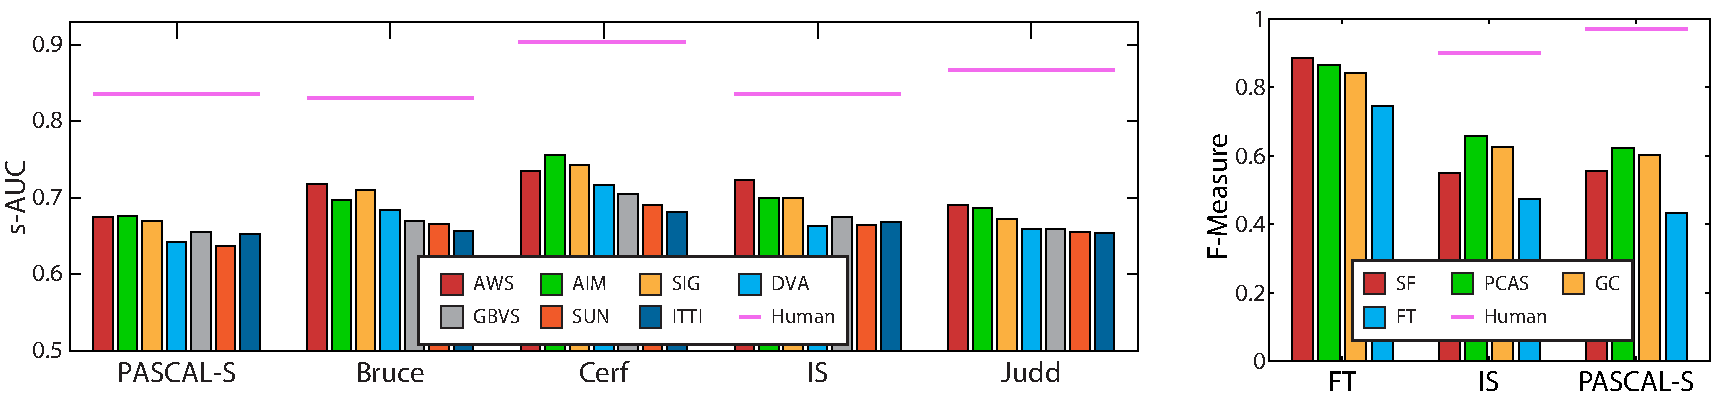
\includegraphics[width=1.0\linewidth]{auc_pr_all2.pdf}\\
\caption{\textbf{Left}: The s-AUC scores of fixation prediction.  \textbf{Right}: The F-Measure scores of salient object segmentation.  According to \cite{achanta2009frequency},  we choose $\beta = 0.3$ to calculate the F-measure from PR curve. In both figures, magenta lines show the inter-subject consistency score of these datasets. These numbers can be interpreted as the upper-bounds of algorithm scores. }\label{fig:fullBench}
\end{figure*}



\subsection{Dataset design bias}
The performance gap among datasets clearly suggests new challenges in salient object segmentation.  However, it is more important to pinpoint the cause to the performance degradation rather than to start benchmark race on another new dataset.  In this section, we analyze the following image statistics in order to find the similarities and differences of today's salient object segmentation datasets:

\begin{figure}[t]
\centering
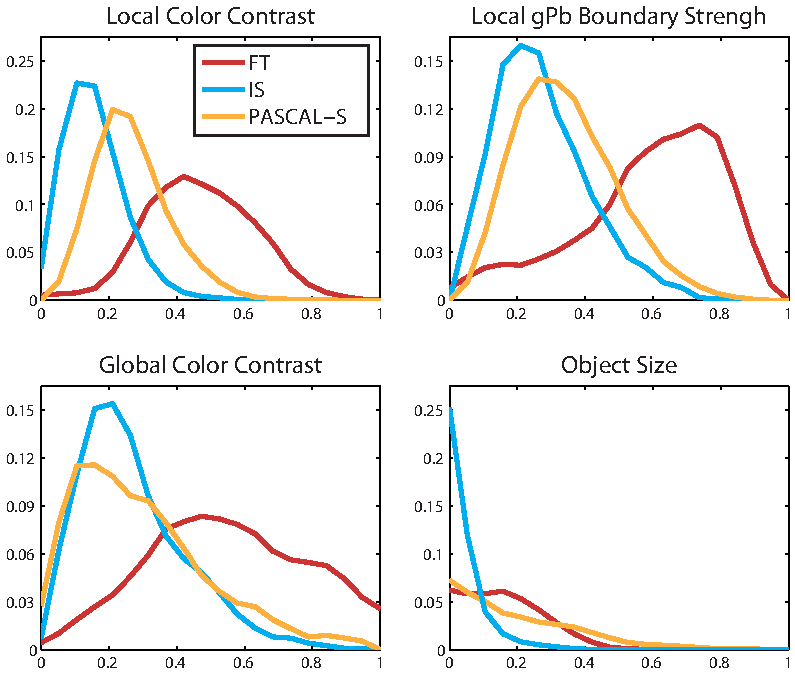
\includegraphics[width=0.7\linewidth]{designBias.pdf}\\
\caption{Image statistics of the salient object segmentation datasets.  The statistics of FT dataset is different from other datasets in local/global color contrast and boundary strength.  As for object size, the PASCAL-S contains a balanced mix of large and small objects.}\label{fig:designBias}
\end{figure}


\begin{description}
\item [Local color contrast:] Segmentation or boundary detection is an inevitable step in most salient objects detectors.  It is important to check whether the boundaries are ``unnaturally'' easy to segment.  To estimate the strength of the boundary, we crop a $5 \times 5$ image patch at the boundary location of each labeled object, and compute RGB color histograms for foreground and background separately.  We then calculate the $\chi^2$ distance to measure the distance between two histograms.  It is worth noting that some of the ground-truth of the IS dataset are not perfectly aligned with objects boundaries, resulting in an underestimate of local contrast magnitude.
\item [Global color contrast:] The term ``saliency'' is also related to the global contrast of the foreground and background.  Similar to the local color contrast measure, for each object, we calculate the $\chi^2$ distance between its RGB histogram and the background RGB histogram.
\item [Local gPB boundary strength:] While color histogram distance captures some low-level image features, an advanced boundary detector, such as gPB \cite{arbelaez2011contour}, combines local and global cues to give a more comprehensive estimate of the presence of a boundary.  As a complementary result to our local color contrast measure, for object boundary pixel we compute the mean gPB response of a $3 \times 3$ local patch.
\item [Object size:] In each image, we define the size of an object as the proportion of pixels in the image.  Most of the objects in IS are very small.
\end{description}


As shown in Fig.~\ref{fig:designBias}, FT dataset stands out in local/global color contrast as well as the gPB boundary strength statistics.  At a first glance, our observation that FT contains unnaturally strong object boundaries seem acceptable, especially for a dataset focusing on salient object analysis.  Strong boundaries are linked to the core concept of saliency: a foreground object with discernable boundaries being surrounded by background that have contrastive colors.  In fact, many images in the FT dataset are textbook examples to demonstrate the definition of saliency.  The notion of ``saliency'' in FT is much less ambiguous than in other datasets.  However, such reduction of ambiguity during the \emph{image selection process} is more destructive rather than constructive, for the purpose to test saliency.  The confusion between image selection process and image annotation process introduces a special kind of bias by over-expressing the desired properties of the target concept, and reduce the presence of negative examples.  We call this type of bias the \emph{dataset design bias}:
\begin{quote}
During the design of a dataset, the image annotation process should be independent of the image selection process.  Otherwise the \emph{dataset design bias} will arise as a result of disproportionate sampling of positive/negative examples.
\end{quote}


\subsection{Fixations and F-measure}
Previous methods of salient object segmentation have reported big margin of F-measures over all fixation algorithms.  However, most of these comparisons are done on the FT dataset, which has shown to have non-negligible dataset bias.  Another factor that contributes to the inferior performance of fixation algorithms is the center-bias.  Major salient object segmentation algorithms, such as SF, PCAS, and GC, have implemented their own treatments for the center-bias.  In contrast, many fixation prediction algorithms, such as AWS and SIG, do not implement center bias as they expect to be benched by s-AUC score which cancels the center-bias effect.  To discount the influence of center-bias, we add a fixed Gaussian ($\sigma = 0.4$ of the image width) to the saliency maps generated by all fixation algorithms, and then benchmark these algorithms on all 3 salient object datasets.  The result is shown in Fig.~\ref{fig:finalResult}.

In addition, we also tested the F-measure of the ground-truth human fixation maps on IS and PASCAL-S.  Each fixation map is blurred by a Gaussian kernel with $\sigma = 0.03$ of the image width.  No center bias is superimposed because the human fixations are already heavily biased towards the center of the image.

When we remove the effect of center bias and dataset design bias, the performance of fixation algorithms becomes very competitive.  We also notice that the F-measure of the ground-truth human fixation maps is rather low compared to the inter-subject consistency scores in the salient object labeling experiment. This performance gap could be either due to a weak correlation between the fixation task and the salient object labeling task, or the incompatibility of the representation of fixations (dots) versus the representation of objects (regions).  In the next section, we will show that the latter is more likely to be true.  Once equipped with appropriate underlying representation, the human fixation map, as well as their algorithm approximations, generate accurate results for salient object segmentation.
